\section{Experimental Results}
\label{sec:experiments}

\begin{comment}
\textcolor{blue}
{Our experiments evaluate three research questions. (1) How does \sys\ perform compared to the baselines when the amount of unseen words in the KB increases?
%(Section \ref{sec:expt1})
, (2) How does the performance of \sys\ compare with existing task-oriented dialog systems?,
%(Section \ref{sec:expt2})? 
And, (3) What is the incremental contribution of each of \sys's components?}
%(Section \ref{sec:expt3})?
\end{comment}

Our experiments evaluate three research questions. 
\begin{compactenum}
    \item \emph{Performance Study}: How well is \sys\ able to perform the tasks of our three datasets as compared to the baseline models? 
    % \item How does \sys\ perform as compared to the baselines on our three datasets?
    \item \emph{Disentanglement Study}: How robust are the models in generalizing on the KA test sets? 
    \item \emph{Ablation Study}: What is the performance gain from each novel feature in \sys? 
\end{compactenum}

\subsection{Performance Study}
\label{sec:expt2}

Table \ref{tab:babi} reports the per-response and per-dialog (in parentheses) accuracies on the bAbI dialog tasks.
% retrieval model comparison
The multi-hop retrieval-based models such as QRN, MN and GMN perform well on the non-OOV test sets for tasks 1, 2, and 5, but fail to exhibit similar performance on the corresponding OOV test sets. This result is expected as these models are trained to retrieve from a pre-defined set of responses. Their poor non-OOV performance on tasks 3 and 4 is attributed to an error in the bAbI dataset construction, due to which, the non-OOV and OOV test conditions are the same for these tasks (see Appendix).

% simple generative model as good accuracy as retrieval
A simple generative model (Seq2Seq) achieves accuracies comparable to the multi-hop retrieval models. Enabling it with the ability to copy from the context (Seq2Seq+Copy) shows a considerable increase in performance, especially on the OOV test sets (and non-OOV tests for tasks 3 and 4).

The strong performance of simple sequence encoders when compared with multi-hop encoders (in retrieval models) raises a question about the value of multi-hop inference. Mem2Seq answers this question, by obtaining improvements in several tasks,  specifically on their OOV test sets. This clearly shows that multi-hop inference and the copy mechanism are essentials for task-oriented dialogs.

% Although Mem2Seq achieves gains, the performance difference between non-OOV and OOV test sets remains large. 
Despite gains from the Mem2Seq model, the performance difference between the non-OOV and OOV test sets remains large. \sys\ succeeds to bridge this gap with its ability to better interpret unseen words, using their surrounding context. It obtains significant improvements on average of about 34\% per-dialog accuracy and 10\% per-response accuracy for the bAbI OOV test sets.

%We also compare against the recently proposed Mem2Seq. As discussed, the primary comparison is against Mem2Seq, which runs the model on unprocessed training data. We also include the numbers with pre-processing (Mem2Seq*) for completeness. 

%The superior performance of \sys\ on OOV tasks is attributed to its ability to capture word's context in an utterance and address any word in the KB tuple.

\begin{table}[t]
\centering
\footnotesize
 \begin{tabular}{l|cc|cc}
\toprule
& \multicolumn{2}{c|}{\textbf{CamRest}} & \multicolumn{2}{c}{\textbf{SMD}}  \\ \cmidrule{2-5}
& \textbf{BLEU} & \textbf{Ent. F1} & \textbf{BLEU} & \textbf{Ent. F1} \\
\midrule
Mem2Seq* & 12.7 & 39 & 12.6 & 33.4  \\
\midrule
Seq2Seq & 11.4 & 40.6 & 8.7 & 34.9  \\
%Seq2Seq+Attn & & & 9.3 & 19.9 \\
Seq2Seq+Copy & 4.7 & 32.2 & 3.23 & 16.9  \\
Mem2Seq & 12.7 & 39 & \textbf{10.3} & 31.8 \\ 
\midrule
\sys\ & \textbf{15.2} & \textbf{43.1} & 8.3 & \textbf{35.9} \\
\bottomrule
\end{tabular}
\caption{Performance of \sys\ and baselines on the CamRest and SMD datasets}
\label{tab:smd}
\end{table}

In Table \ref{tab:smd}, we report results on the real-world datasets. \sys\ greatly outperforms other models in both Entity F1 metric and BLEU scores on CamRest. On SMD, \sys\ achieves the best only in Entity F1. On further analysis of the generated responses we observe that \sys\ responses often convey the necessary entity information from the KB. However, they consist of meaningful phrases with little lexical overlap with the gold response, reducing the BLEU scores. We investigate this further in our human evaluation.

%We noticed that the reported results for Mem2Seq are not directly comparable, as they pre-processed training data in dataset-specific ways. For direct comparisons, we re-run Mem2Seq on the original training datasets \footnote{Mem2Seq used the following pre-processing on the data: 1) The subject (restaurant name) and object (rating) positions of the rating KB tuples in bAbI dialogs are flipped 2) an extra fact was added to the navigation tasks in In-Car Assistant with all the properties (such as distance, address) combined together  as the subject and \textit{poi} as the object. We evaluated Mem2Seq by removing these pre-processing steps.} and repeat all experiments. For completeness we also mention their reported results (with pre-processing) as Mem2Seq*. 
\noindent \textbf{Human Evaluation:}
%Our first human evaluation experiment aims to measure the ability of the generated response to pass on relevant information to the user towards solving the task. We obtain a total of 100 annotations per system per test set on both Camrest and SMD, 2 each for 50 randomly sampled dialogs. We ask the annotators to label accuracy of the information. In second experiment,  we check for grammatical coherence  asking the annotator to rate each response on a scale of 0(bad)-3(good) based on the fluency and correctness of the response.
We summarize the human evaluation results for real-world datasets in Table \ref{tab:amt_perf}. \sys\ shows the best performance on Camrest, and is judged useful 77 times out of 100. Also, it has the highest average grammatical correctness score of 2.28 (very close to Seq2Seq and Mem2Seq). \sys\ performs on par with Mem2Seq and Seq2Seq in its ability to relay appropriate information to solve SMD dialog tasks, and has a slightly higher grammaticality score.

\begin{table}[t]
\centering
\footnotesize
 \begin{tabular}{l|cc|cc}
\toprule
& \multicolumn{2}{c|}{\textbf{CamRest}} & \multicolumn{2}{c}{\textbf{SMD}}  \\ \cmidrule{2-5}
& \textbf{Info} & \textbf{Grammar} & \textbf{Info} & \textbf{Grammar} \\
\midrule
Seq2Seq & 46 & 2.24 & 35 &  2.38 \\
Seq2Seq+Copy & 27 & 1.1 & 21 &  1.04 \\
Mem2Seq & 51 & 2.2 & \textbf{38} &  2.0 \\
\midrule
\sys\ & \textbf{77} & \textbf{2.28} & 36 &  \textbf{2.5} \\

\bottomrule
\end{tabular}
\caption{AMT Evaluations on CamRest and SMD} 
\label{tab:amt_perf}
\end{table}

\begin{comment}
Table \ref{tab:smd} reports the results on DSTC2. \sys\ exhibits performance comparable to other models. As the data was generated by humans interacting with bots, it contains significant noise introduced by the bot. For example, in one of the training examples, the bot responds with "You are looking for a restaurant is that right\?" when the human requested for phone number of a restaurant. This inherent difficulty in the data makes it harder to model.
\end{comment} 

\subsection{Disentanglement Study}
\label{sec:expt1}
We use our generated knowledge adaptability (KA) test sets to measure the robustness of \sys\ and the other baselines to changes in the KB. We perform this experiment on 4 different tasks, namely bAbI tasks 1 and 5, CamRest, and SMD.

Figures \ref{label-a} and \ref{label-b} show the per-response accuracies of the two bAbI dialog tasks plotted against the percentage of unseen entities in KA sets. From Figure \ref{label-a} we observe that \sys\ remains immune to any variablity in the KB content, whereas the performance of Mem2Seq and Seq2Seq models drops drastically due to their inability to capture semantic representations of the injected KB entities. We see a similar trend in Figure \ref{label-b}, but here all the models show a drop in performance, with \sys\ appearing the most steady. We explain this trend using the example dialog in Table \ref{tab:t5_dis}. In the current dialog context, the system is required to provide the address of the selected restaurant, but since more than one restaurant in the KB is unseen, it becomes ambiguous for the network to identify the correct restaurant and infer its address. In the end, the system is forced to pick a random address -- the probability of which being correct decreases as more restaurants become unseen.

\begin{table}[!t]
\centering
\scriptsize
\begin{tabular}{c|l}
\toprule
%\textbf{kb} & \textit{da\_vinci\_pizzeria}\\
% & \textit{r_phone|01223\_351707} \\
% & \textit{r_adddress|20\_milton\_road\_chesterton} \\
% & \textit{r_food|italian} \\
\multicolumn{2}{c}{\textbf{KB (restaurant|address)}} \\
\multicolumn{2}{c}{\textit{r\_bangkok\_overpriced\_thai\_8}|\textit{r\_bangkok\_overpriced\_thai\_8\_addr}}\\
\multicolumn{2}{c}{\textit{r\_bangkok\_overpriced\_thai\_7}|\textit{r\_bangkok\_overpriced\_thai\_7\_addr}}\\
\multicolumn{2}{c}{\textit{r\_bangkok\_overpriced\_thai\_4}|\textit{r\_bangkok\_overpriced\_thai\_4\_addr}}\\
\multicolumn{2}{c}{\textit{r\_bangkok\_overpriced\_thai\_2}|\textit{r\_bangkok\_overpriced\_thai\_2\_addr}}\\
\midrule
\midrule
\textbf{usr-1} & may i have a table in an \textit{overpriced} price range for \\
& \textit{nine} people with \textit{thai} food in \textit{bangkok} ? \\
\textbf{sys-1} & what do you think of : \textit{r\_bangkok\_overpriced\_thai\_8} ? \\
\textbf{usr-2} & can you provide the address ? \\
\midrule
\textbf{Gold} & here it is \textit{r\_bangkok\_overpriced\_thai\_8\_addr}
 \\
\midrule
\midrule
\textbf{Seq2Seq+Copy} & here it is \textit{r\_bangkok\_overpriced\_thai\_4\_addr}
 \\
\midrule
\textbf{Seq2Seq} & here it is \textit{r\_london\_moderate\_spanish\_6\_addr} \\

\midrule
\textbf{Mem2Seq} & here it is \textit{r\_bangkok\_overpriced\_thai\_4\_addr} \\
\midrule
\textbf{\sys\ } & here it is \textit{r\_bangkok\_overpriced\_thai\_4\_addr} \\
\bottomrule
\end{tabular}
\caption{Example from bAbI Task 5 KA test set with 100\% OOV entities. Identifying the address of an unseen restaurant is challenging for all models.}
\label{tab:t5_dis}
\end{table}

The performance on the CamRest KA test sets is illustrated in Figures \ref{fig:camrest} and \ref{label-c}. \sys\ has the best performance with even a slight increase in both BLEU and Entity F1 metrics as more OOV content is injected in the dialog, probably because it is clear that it needs to copy when processing unseen entities.
% We speculate that because CamRest consists of relatively short dialogs, the ability to inference is more profound and the model is successfully able to copy the OOV entity. Moreover, when the system encounters an unseen word, it is certain to copy and due to less confusion in deciding to generate or copy the word, \sys\ is able to give increased performance. 
Seq2Seq+Copy is unable to perform well in CamRest as the length of the input (dialog history + KB tuples) is long and the size of the training set is also small. We believe that Seq2Seq+Copy works best in an environment with an abundance of short dialog training data (e.g., bAbI task 1 in Figure \ref{label-a}).

SMD consists of dialogs with a large KB and a highly varying response pattern. This makes it very difficult to learn the language model -- reflected in the low BLEU scores for all the systems. \sys\ still provides the best F1 entity score due to its ability to inference efficiently on the large KB (Figure \ref{label-d}). Mem2Seq shows the best BLEU score performance on the original test set, but its performance drop of 42.5\%, from 10.3 at 0\% unseen to 5.93 at 100\% unseen, is a lot heavier than that of \sys\ which only drops 7.6\% -- 8.27 at 0\% unseen to 7.64 at 100\% unseen.

\noindent \textbf{Human Evaluation:}
We summarize the human evaluation results for real-world datasets on the 50\% unseen KA test set in Table \ref{tab:amt_dis}. \sys\ again outperforms the baselines and is labeled \emph{successful} twice more often than the next best model on both Camrest and SMD. Seq2Seq appears to produce better sentence structures on the SMD dataset, primarily because it does not attempt to learn inference on the KB, allowing it to solely focus on learning the language model better. 

\begin{table}[t]
\centering
\footnotesize
 \begin{tabular}{l|cc|cc}
\toprule
& \multicolumn{2}{c|}{\textbf{CamRest}} & \multicolumn{2}{c}{\textbf{SMD}}  \\ \cmidrule{2-5}
& \textbf{Info} & \textbf{Grammar} & \textbf{Info} & \textbf{Grammar} \\
\midrule
Seq2Seq & 26 & 2.28 & 22 & \textbf{2.44} \\
Seq2Seq+Copy & 22 & 1.22 & 16 & 1.04 \\
Mem2Seq & 35 & 2.06 & 26 & 1.9 \\
\midrule
\sys\ & \textbf{80} & \textbf{2.44} & \textbf{51} &  2.28 \\

\bottomrule
\end{tabular}
\caption{AMT Evaluations on CamRest and SMD (50\% unseen) KA datasets} 
\label{tab:amt_dis}
\end{table}


% \begin{table}[t]
% \centering
% \footnotesize
%  \begin{tabular}{l|cc|c|cc|c}
% \toprule
% & \multicolumn{3}{c|}{\textbf{CamRest676}} & \multicolumn{3}{c}{\textbf{SMD}}  \\ \cmidrule{2-7}
% & \textbf{0\%} & \textbf{50\%} & \textbf{Total} & \textbf{0\%} & \textbf{50\%} & \textbf{Total} \\
% \midrule
% Seq2Seq & 46 & 26 & 72 & 35 & 22 & 57 \\
% Seq2Seq+Copy & 27 & 22 & 49 & 21 & 16 & 37 \\
% Mem2Seq & 51 & 35 & 86 & \textbf{38} & 26 & 64 \\
% \midrule
% \sys\ & \textbf{77} & \textbf{80} & \textbf{157} & 36 & \textbf{51} & \textbf{87} \\

% \bottomrule
% \end{tabular}
% \caption{AMT Evaluations on CamRest676 and In-car Assistant datasets} 
% \label{tab:amt}
% \end{table}

% \begin{table}[t]
% \centering
% \footnotesize
%  \begin{tabular}{l|cc|cc}
% \toprule
% & \multicolumn{2}{c|}{\textbf{CamRest676}} & \multicolumn{2}{c}{\textbf{SMD}}  \\ \cmidrule{2-5}
% & \textbf{0\%} & \textbf{50\%} &  \textbf{0\%} & \textbf{50\%}\\
% \midrule
% Seq2Seq & 2.24 & 2.28 & 2.38 & \textbf{2.44} \\
% Seq2Seq+Copy & 1.1 & 1.04 & 2.0 & 1.04 \\
% Mem2Seq & 2.2 & 2.06 & 2.0 & 1.9  \\
% \midrule
% \sys\ & \textbf{2.28} & \textbf{2.44} & \textbf{2.5} & 2.28 \\


% \bottomrule
% \end{tabular}
% \caption{AMT Grammar Evaluations on CamRest676 and In-car Assistant datasets} 
% \label{tab:amtg}
% \end{table}

\begin{figure*}
\centering
\begin{minipage}[b]{.475\textwidth}
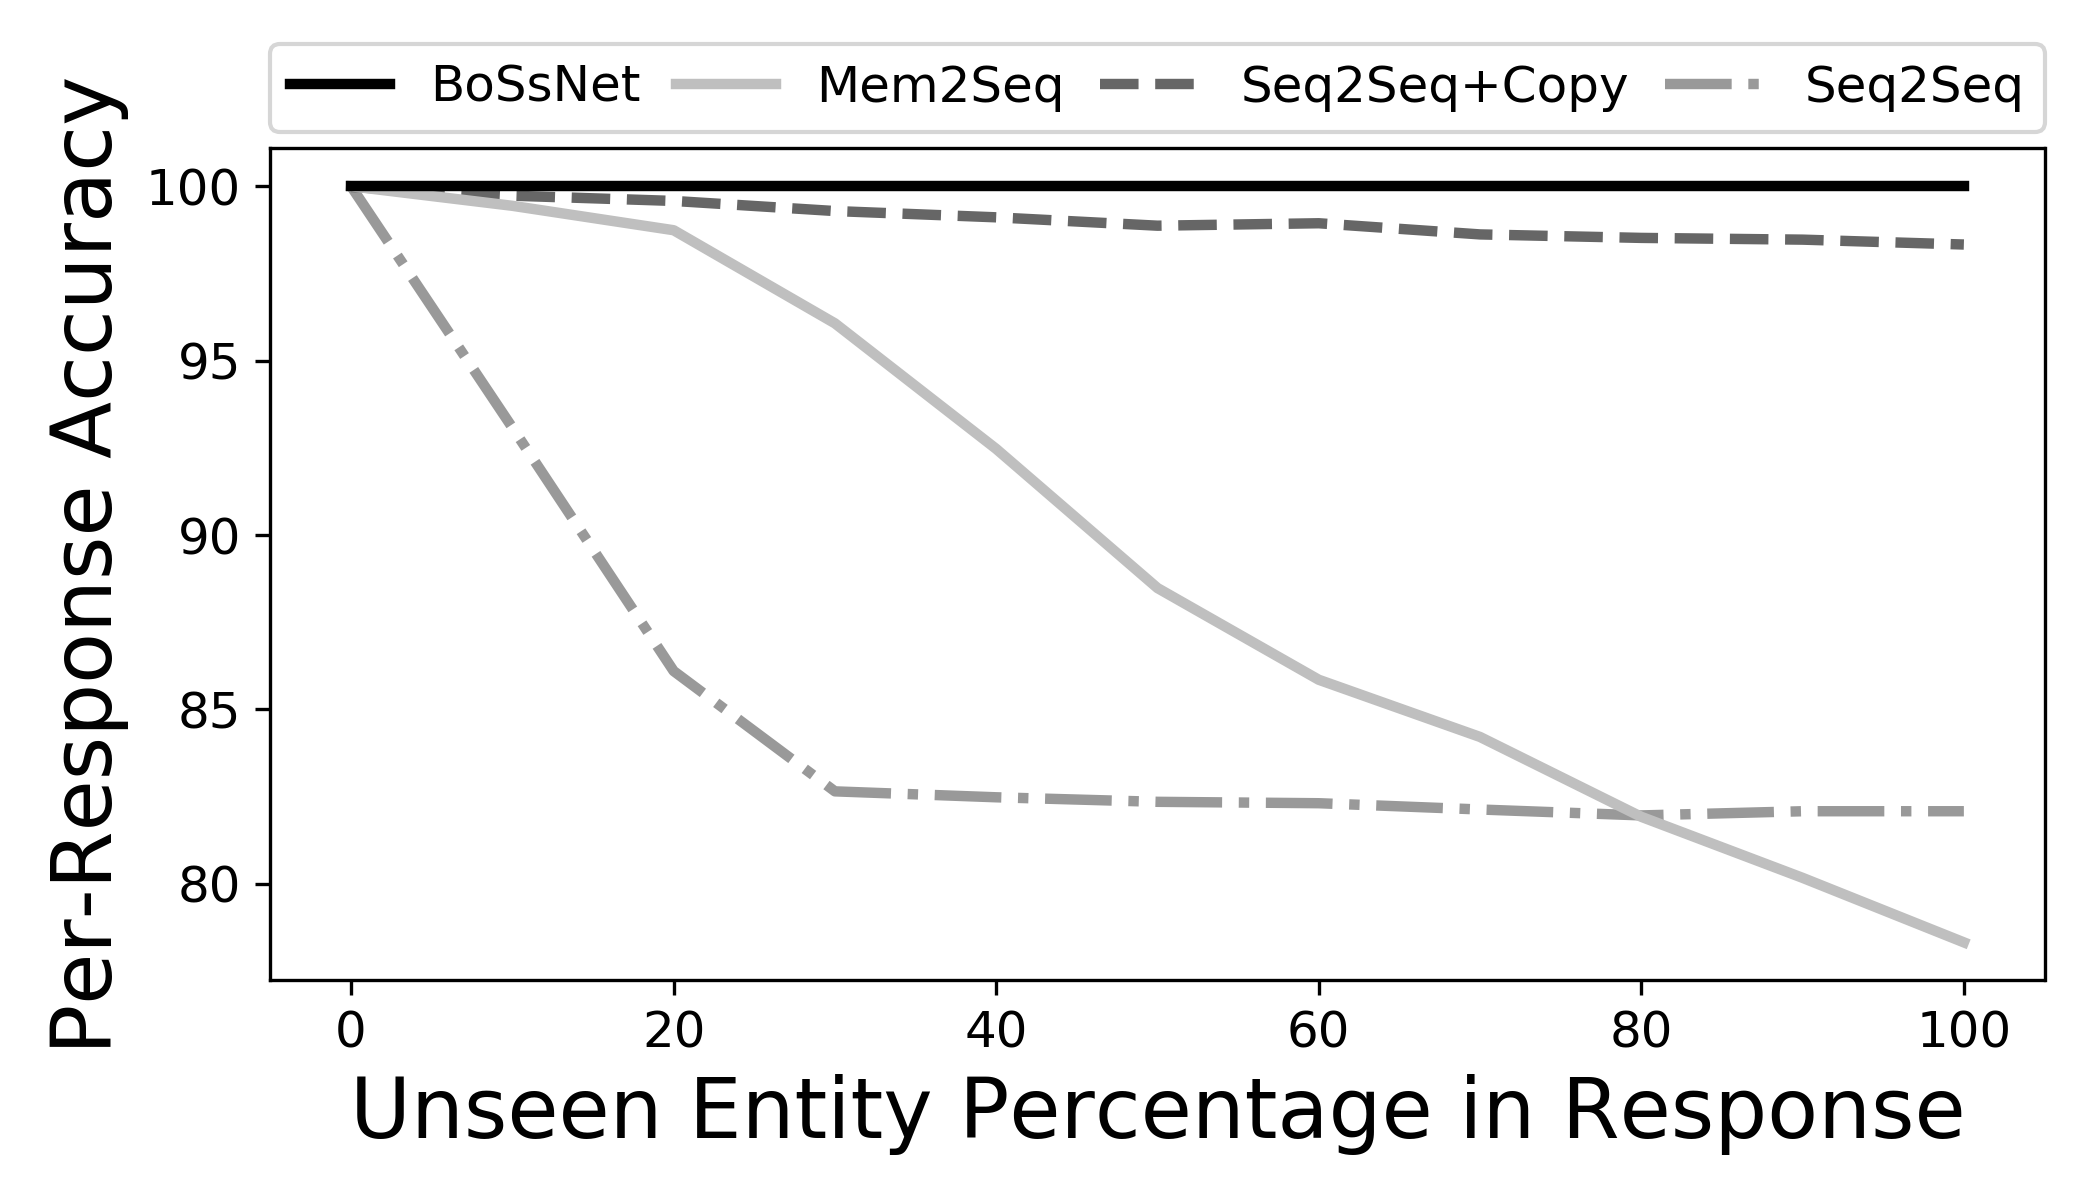
\includegraphics[width=\textwidth, height=4.7cm]{assets/graphs/task1_Acc.png}
\caption{bAbI Task 1: Per-response accuracy comparison on KA sets}\label{label-a}
\end{minipage}\qquad
\begin{minipage}[b]{.475\textwidth}
 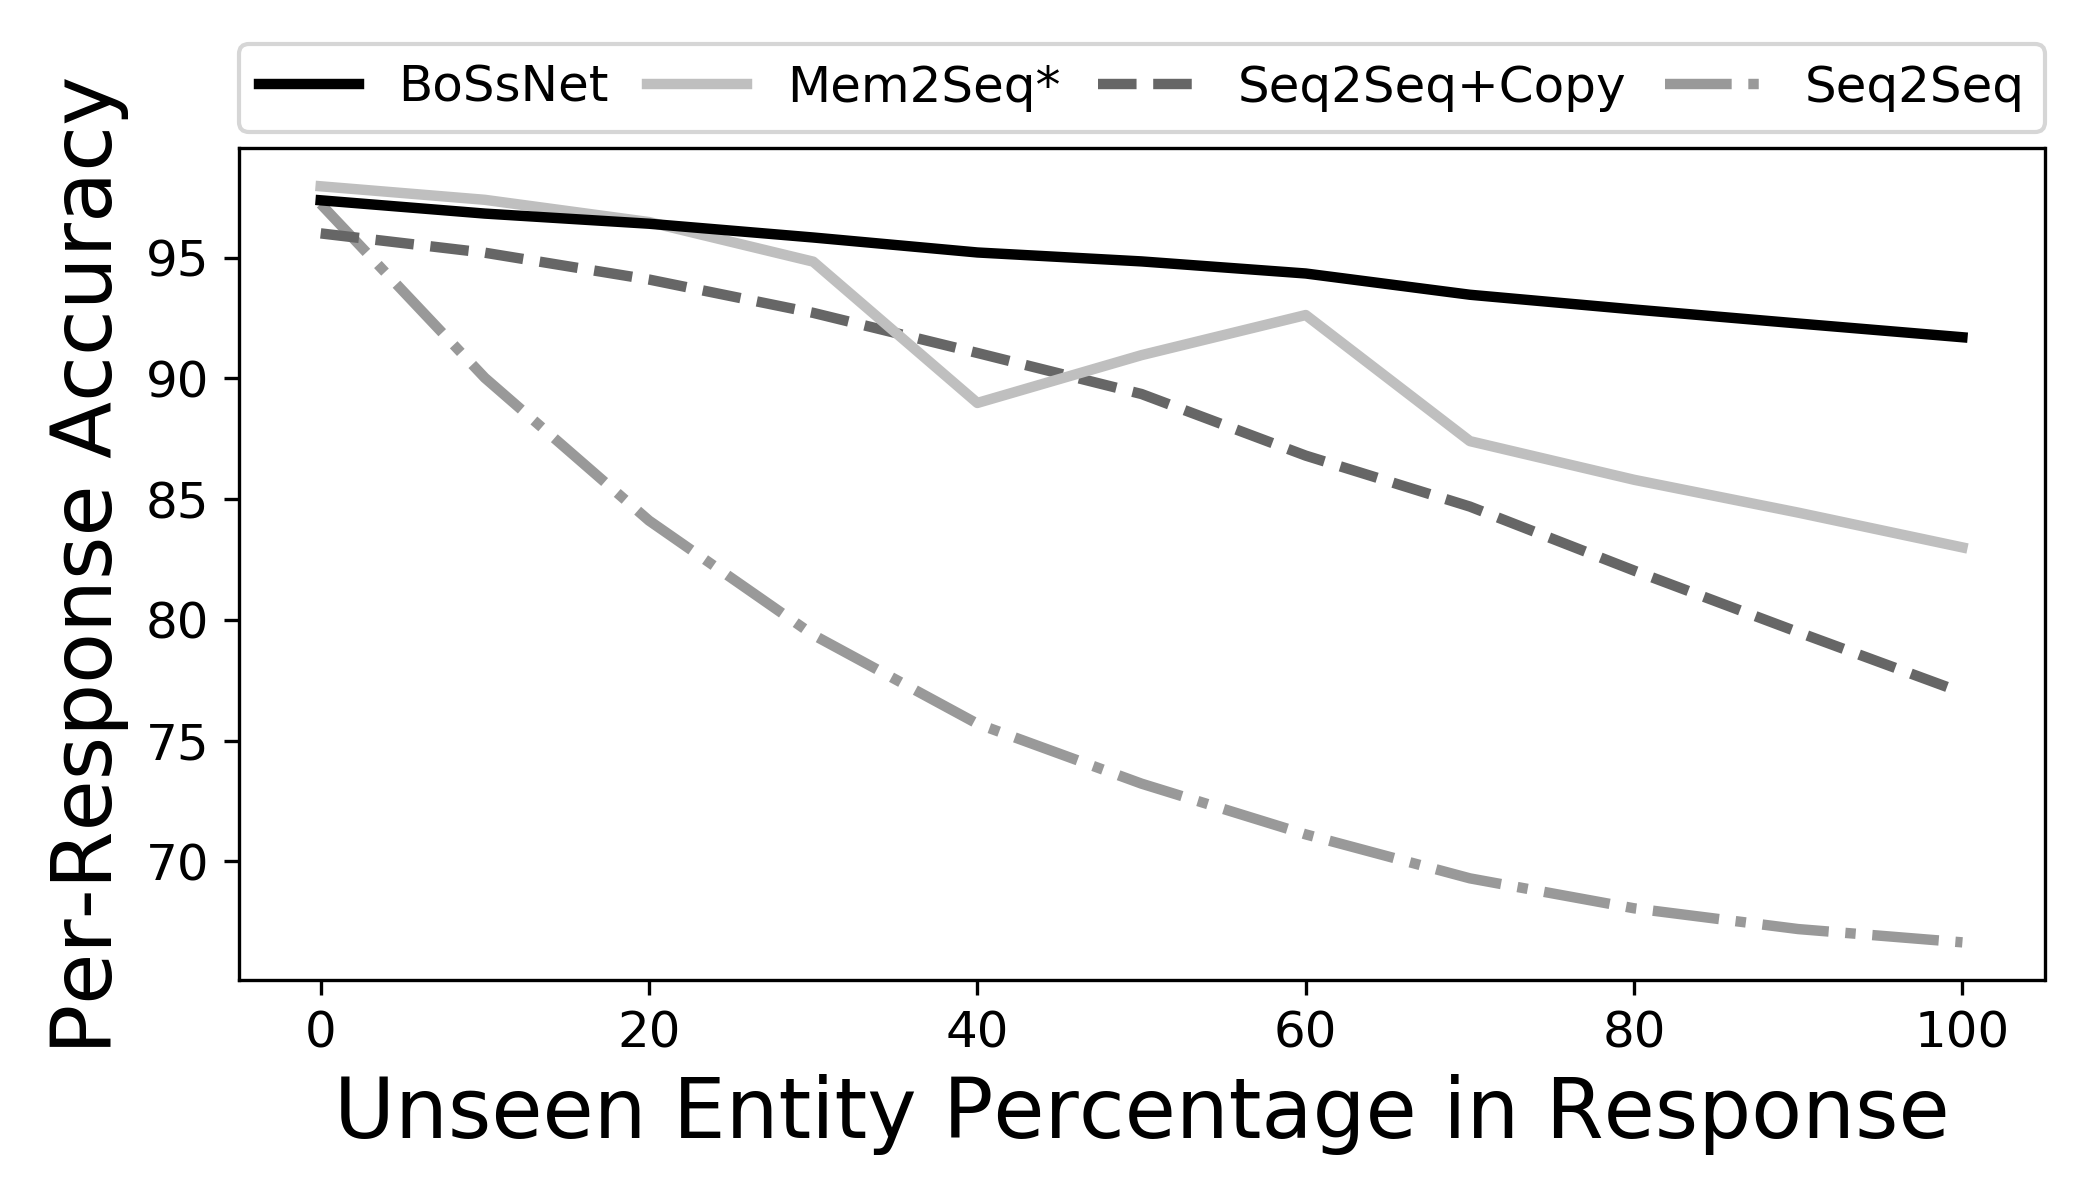
\includegraphics[width=\textwidth, height=4.7cm]{assets/graphs/task5_Acc.png}
        \caption{bAbI Task 5: Per-response accuracy comparison on KA sets}\label{label-b}
\end{minipage}
\end{figure*}

\begin{figure*}
\centering
\begin{minipage}[b]{.475\textwidth}
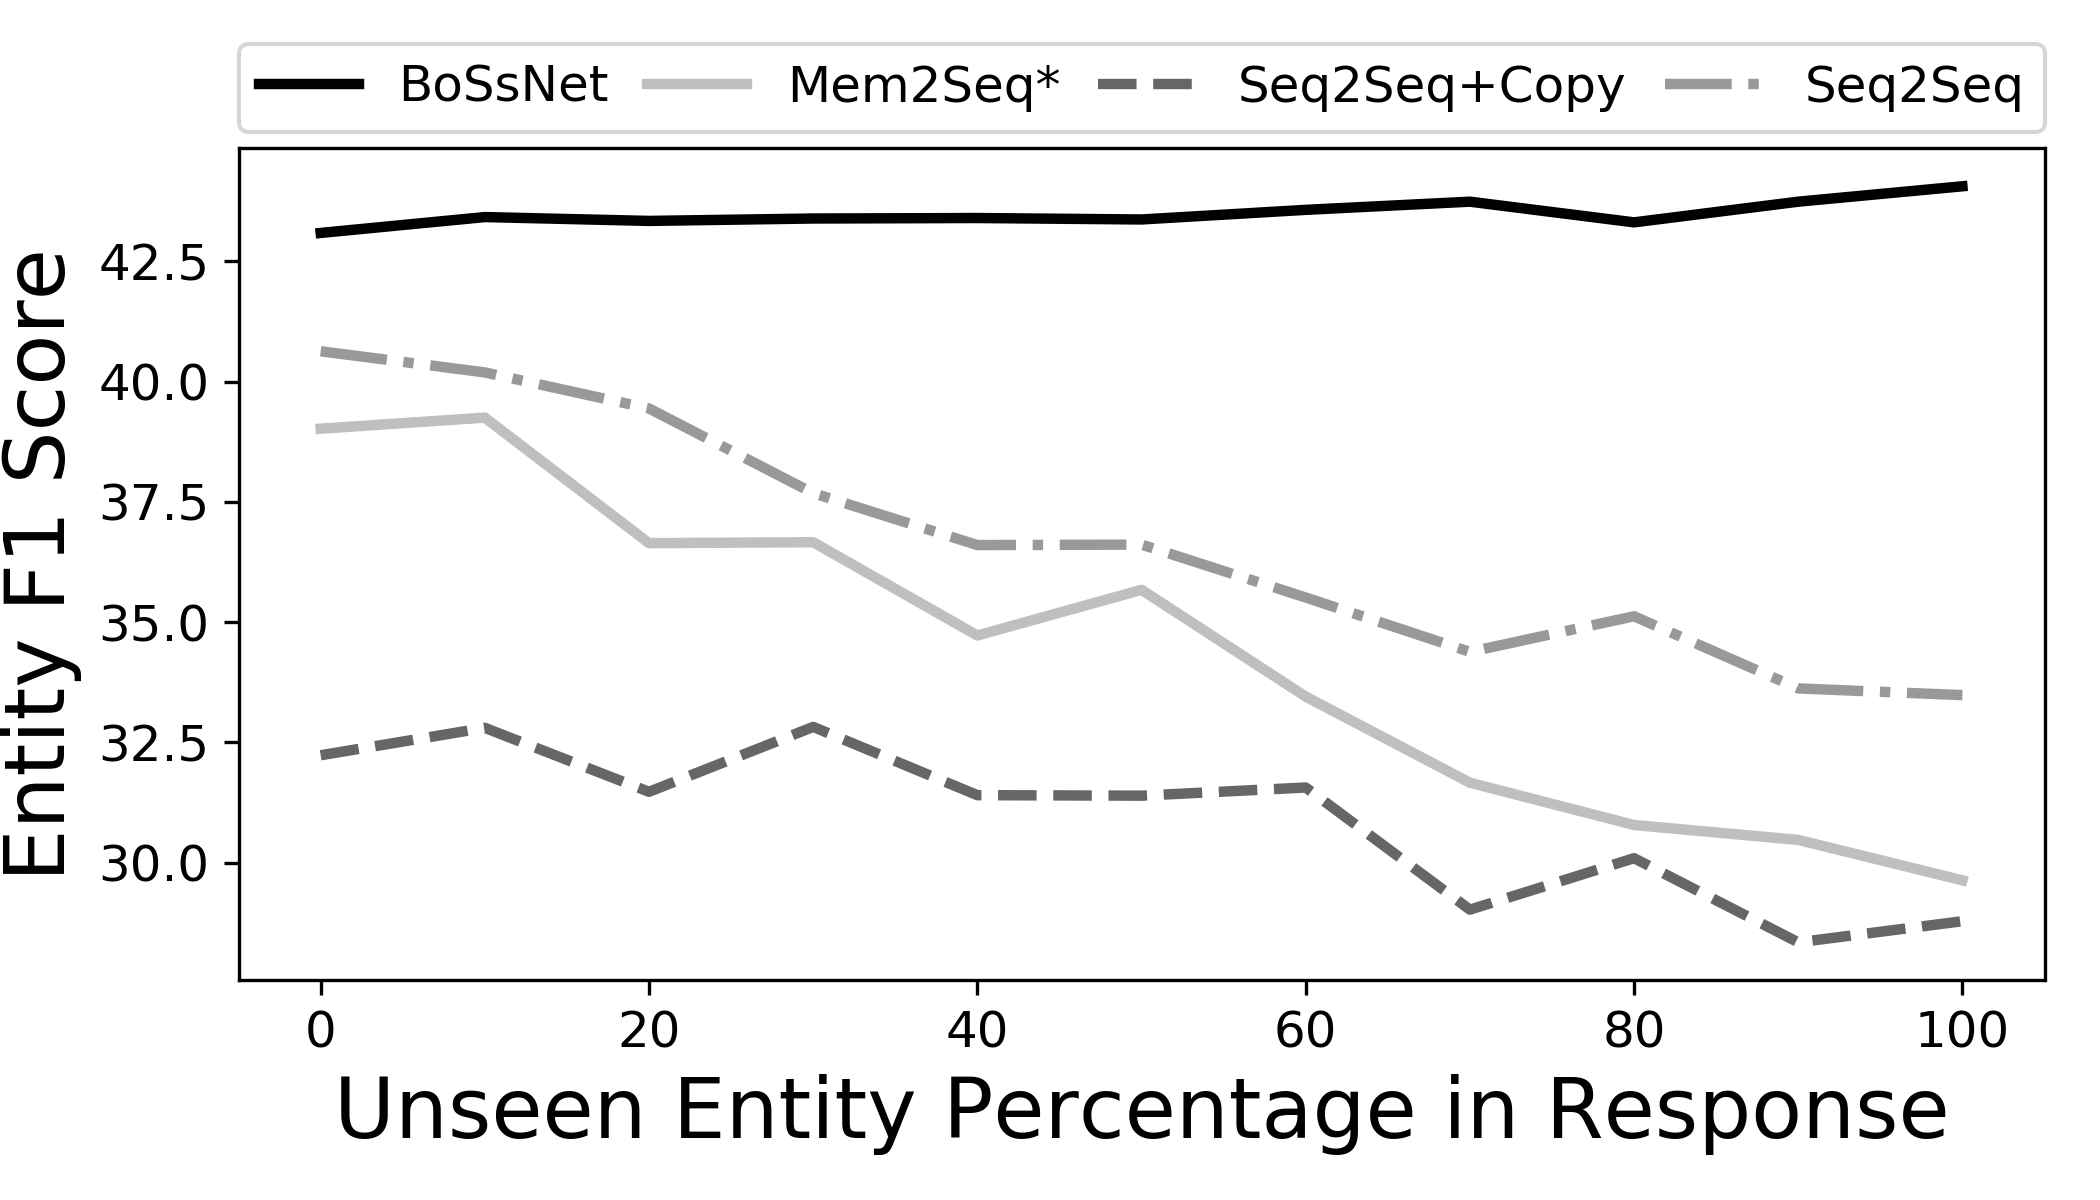
\includegraphics[width=\textwidth, height=4.7cm]{assets/graphs/camrest_F1.png}
\caption{CamRest: Entity F1 comparison on KA sets}\label{label-c}
\end{minipage}\qquad
\begin{minipage}[b]{.475\textwidth}
 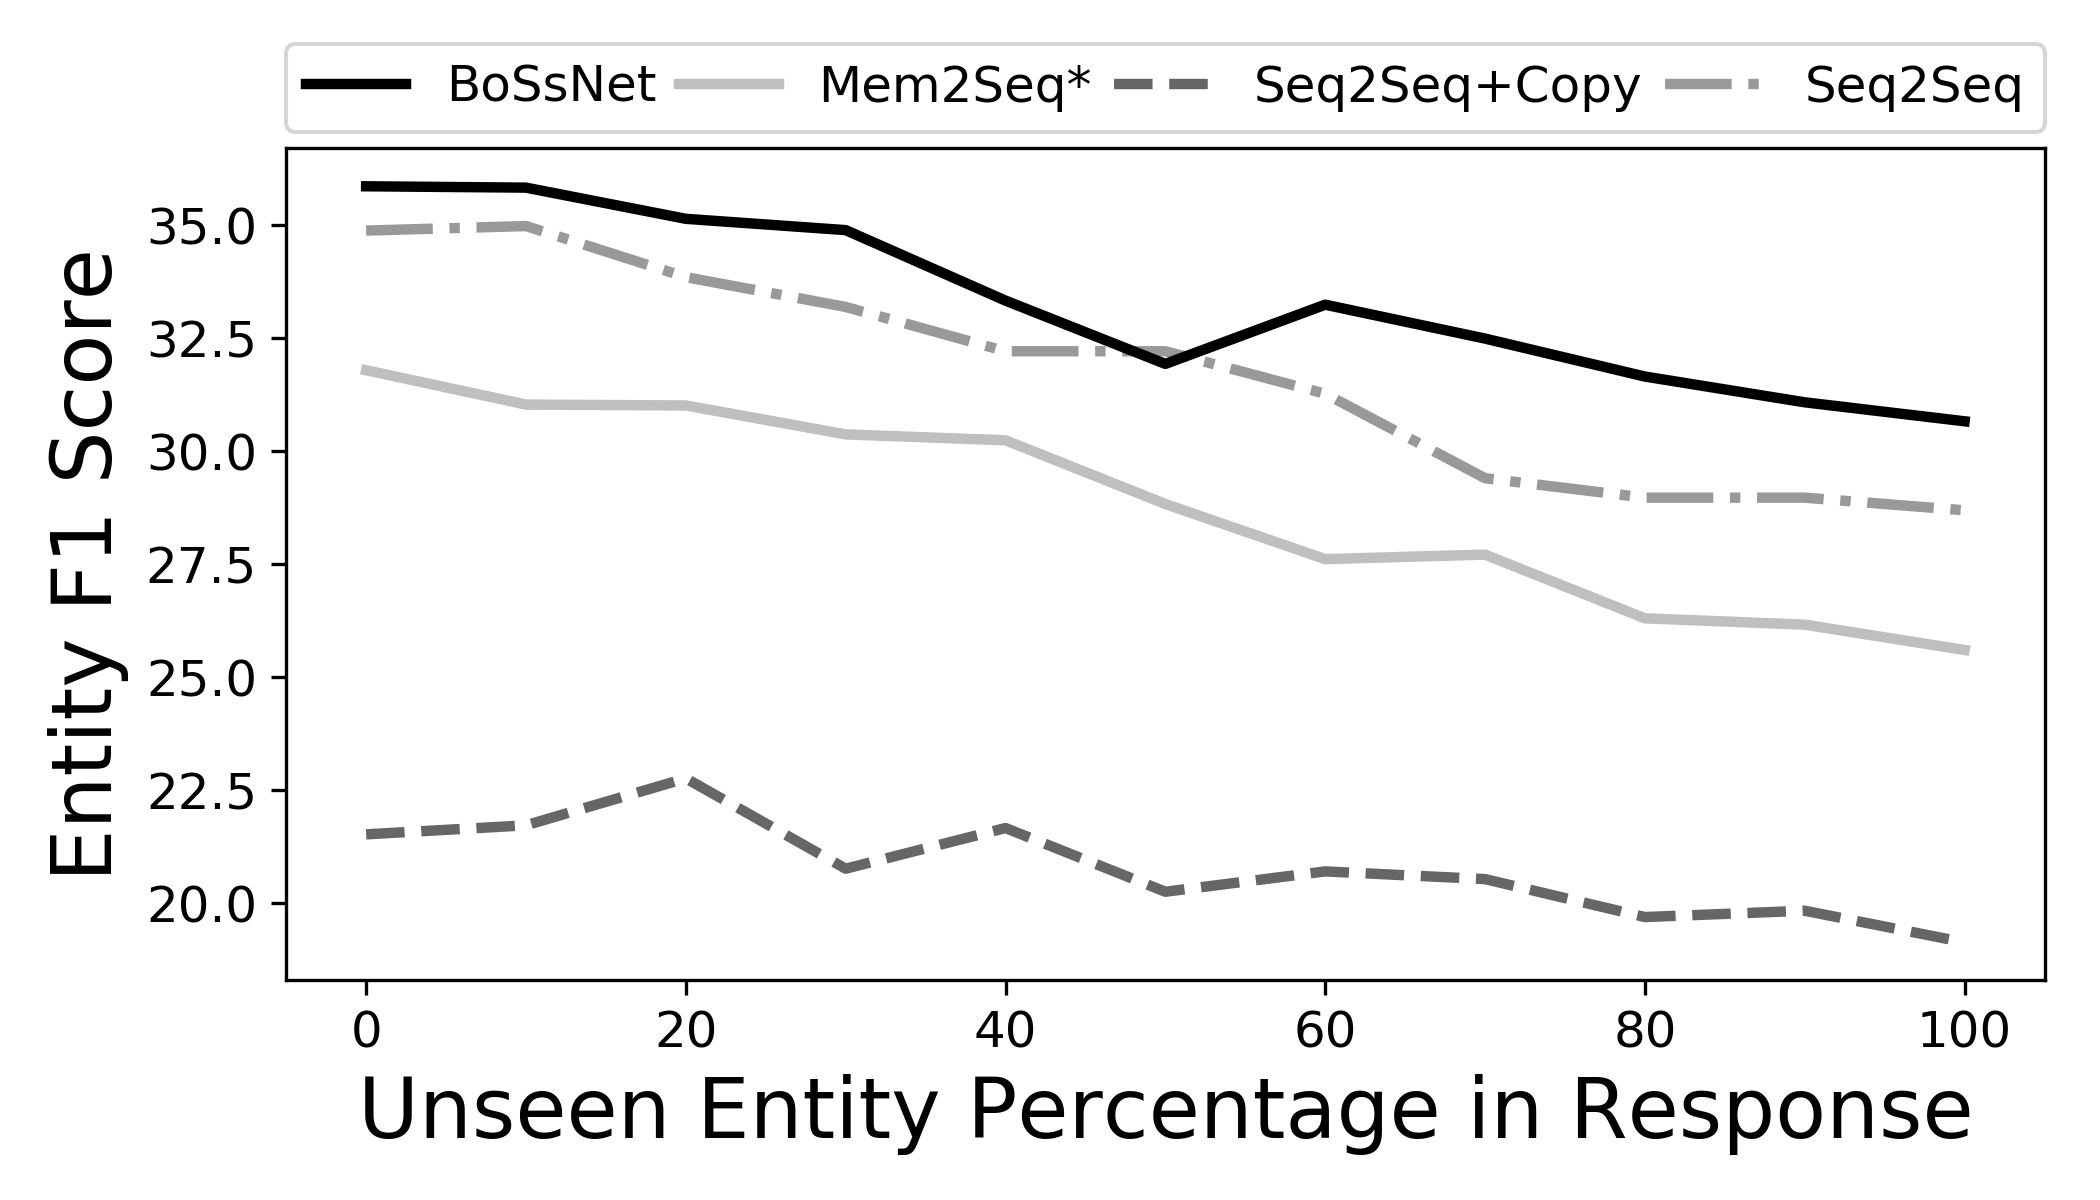
\includegraphics[width=\textwidth, height=4.7cm]{assets/graphs/smd_F1.png}
\caption{SMD: Entity F1 comparison on KA sets}\label{label-d}
\end{minipage}
\end{figure*}

\subsection{Ablation Study}
\label{sec:expt3}

\begin{table*}[!ht]
\centering
\footnotesize
% \vspace{2mm}
\begin{tabular}{l|ccccc|ccccc|cc}
\toprule
   & \multicolumn{5}{c|}{\textbf{bAbI Dialog Tasks}} & \multicolumn{5}{c|}{\textbf{bAbI Dialog Tasks (OOV)}}  & \multicolumn{2}{c}{\textbf{CamRest}} \\ \cmidrule{2-6} \cmidrule{7-11} \cmidrule{12-13}
    & T1  & T2  & T3   & T4   & T5   & T1 & T2 & T3 & T4 & T5 & BLEU        & Ent. F1       \\ \midrule
\sys\ w/o {\sc BoSs} Memory & 100 & 100 & 74.9 & 57.2 & 95.6 & 93.5   & 78.9   & 74.9   & 57     & 81.4   & 10.13        & 29          \\
\sys\ w/o $\mathcal{L}_{d}$          & 100 & 100 & 91.7 & 100  & 94.3 & 83.2   & 78.9   & 92.7   & 100    & 66.7   & 15.5        & 40.1          \\
\sys\  w/o DLD     & 100 & 100 & 93.4 & 100  & 95.3 & 79.2   & 84.6   & 90.7   & 100    & 78.1   & 12.4        & 40.45         \\ \midrule
\sys\                 & 100 & 100 & 95.2 & 100  & 97.3 & 100    & 100    & 95.7   & 100    & 91.7   & 15.2        & 43.1    
\\ \bottomrule
\end{tabular}
\caption{Ablation study: impact of each model element on \sys\ }
\label{tab:ablation}
\end{table*}

\begin{table*}[!ht]
\centering
\footnotesize
% \vspace{2mm}
\begin{tabular}{l|c|c|c}
\toprule
   & \textbf{bAbI Dialog} & \textbf{bAbI Dialog (OOV)}  & \textbf{CamRest} \\ \cmidrule{2-4}
    & Avg. Response Acc.  & Avg. Response Acc. & Ent. F1       \\ \midrule
\sys\ w/o {\sc BoSs} Memory & 85.54 & 77.14 & 29          \\
\sys\ w/o $\mathcal{L}_{d}$          & 97.2 & 84.3 & 40.1          \\
\sys\  w/o DLD     & 97.74 & 86.52 & 40.45         \\ \midrule
\sys\                 & 98.5    & 97.48 & 43.1    
\\ \bottomrule
\end{tabular}
\caption{Ablation study: impact of each model element on \sys\ }
\label{tab:ablation}
\end{table*}

We assess the value of each model element, by removing it from \sys. Table \ref{tab:ablation} reports the per-response accuracy scores for various configurations of \sys\ on bAbI dialog tasks. It also reports the BLEU and entity F1 metric of various configurations on CamRest.

\noindent \textbf{Without BoSs Memory:} 
This configuration uses the Bag-of-Bags (BoB) Memory rather than {\sc BoSs} memory. The BoB memory is a simplified representation, similar to the one in the original Memory Networks. Here the token representation is the vector embedding of the token with no influence from the surrounding words and the memory cell representation is the sum of all its token embeddings. As a result, each word $w$ representation is influenced equally by all words in a memory cell, irrespective of its distance from $w$. This makes capturing context in the immediate neighbourhood harder. Inability to capture the correct context prevents the configuartion from generalizing to OOV test sets.

\noindent \textbf{Without Disentangled Loss:} Disentangled Loss ($\mathcal{L}_{d}$) plays an important role in enforcing that KB words be copied and other language be generated. By removing this loss component, 
%the system will not enforce copying only KB words in the response. When compared with \sys, 
it achieves better BLEU score in CamRest, but with a drop in Entity F1. Without the disentangled loss, the model sometimes learns to generate KB words. This severely affects OOV performance. As described earlier, an error in bAbI dataset construction tasks 3 and 4 effectively injects the validation set with a lot of OOVs. This anomaly in conjunction with the dropout (DLD), helps the configuration in achieving an acceptable performance for those tasks.

\noindent \textbf{Without Disentangled Label Dropout:} 
\sys\ learns to generate language and copy KB words. Without DLD, the model learns to memorize words to be copied rather than learning the context under which a word should be copied. Hence, the performance on OOV test sets is much inferior compared to the non-OOV setting.

Overall, we notice that combining all three model elements is necessary in obtaining the best performance across all tasks.

%We finally see that, the OOV performance is as comparable to the non-OOV performance when all the elements of \sys\ are combined together.

\subsection{Qualitative Evaluation}
We qualitatively compare the performance of \sys\ with other baselines using examples.

Table \ref{tab:camrest-qualeval}, demonstrates the ability of \sys\ to copy entities (restaurant name and address) in its response. The other baselines either generate unwanted or irrelevant entities in their response, or fail to copy altogether. \sys\ also best captures the language model effectively with a slight paraphrasing of the gold response.

Table \ref{tab:task5-qualeval} contains only unseen entities. This example highlights the shortcomings of the Seq2Seq model as it ends up predicting a restaurant encountered during training. Mem2Seq copies a restaurant name without learning to sort the restaurants based on rating. \sys, with its efficient memory addressing, is seen to be able to solve both issues.

\begin{table*}[h]
\centering
\small
\begin{tabular}{c|p{13cm}}
\toprule
%\textbf{kb} & \textit{da\_vinci\_pizzeria}\\
% & \textit{r_phone|01223\_351707} \\
% & \textit{r_adddress|20\_milton\_road\_chesterton} \\
% & \textit{r_food|italian} \\
\multicolumn{2}{c}{\textbf{KB (restaurant|cuisine|address|phone)}} \\
\multicolumn{2}{c}{\textit{pizza\_hut\_fen\_ditton}|\textit{italian}|\textit{cambridge\_retail\_park\_newmarket\_road\_fen\_ditton}|\textit{01223\_323737}}\\
\midrule
\midrule
\textbf{usr-1} & may i have information for an \textit{italian} restaurant in the \textit{east} part of town ? \\
\textbf{sys-1} & yes sure . there is only on \textit{italian} restaurant called \textit{pizza\_hut\_fen\_ditton} in the \textit{east} . what else do you want to know ? \\
\textbf{usr-2} & what is their address please ? \\
\midrule
\textbf{Gold} & the address for \textit{pizza\_hut\_fen\_ditton} is \textit{cambridge\_retail\_park\_newmarket\_road\_fen\_ditton} . can i help you with anything else ?
 \\
\midrule
\midrule
\specialcell[t]{\textbf{Seq2Seq+Copy}} & their address is at
 \\
\midrule
\textbf{Seq2Seq} & \textit{curry\_prince} is at \textit{451\_newmarket\_road\_fen\_ditton} \\

\midrule
\textbf{Mem2Seq} & \textit{pizza\_hut\_fen\_ditton} is located at \textit{7\_barnwell\_road\_fen\_ditton} is \textit{7\_barnwell\_road\_fen\_ditton} and the phone number is \textit{01223\_244955}
 \\
\midrule
\textbf{\sys\ } & \textit{pizza\_hut\_fen\_ditton} is located at \textit{cambridge\_retail\_park\_newmarket\_road\_fen\_ditton} is there anything else i can help you with \\
\bottomrule
\end{tabular}
\caption{An example of responses generated by \sys\ and baselines on the CamRest test set. Thia example has no unseen entities.}
\label{tab:camrest-qualeval}
\end{table*}

\begin{table*}
\centering
\small
\begin{tabular}{c|l}
\toprule
\multicolumn{2}{c}{\textbf{KB (restaurant|cuisine|price\_range|location|rating)}} \\
\multicolumn{2}{c}{\textit{resto\_tokyo\_affordable\_vietnamese\_8stars}|\textit{vietnamese}|\textit{affordable}|\textit{tokyo}|\textit{8}}\\
\multicolumn{2}{c}{\textit{resto\_tokyo\_affordable\_vietnamese\_7stars}|\textit{vietnamese}|\textit{affordable}|\textit{tokyo}|\textit{7}}\\
\multicolumn{2}{c}{\textit{resto\_tokyo\_affordable\_vietnamese\_6stars}|\textit{vietnamese}|\textit{affordable}|\textit{tokyo}|\textit{6}}\\
\multicolumn{2}{c}{\textit{resto\_tokyo\_affordable\_vietnamese\_5stars}|\textit{vietnamese}|\textit{affordable}|\textit{tokyo}|\textit{5}}\\
\midrule
\midrule
\textbf{usr-1} & can you book a table in \textit{tokyo} with \textit{vietnamese} food in a \textit{affordable} price range ? \\
\textbf{sys-1} & what do you think of this option : \textit{resto\_tokyo\_affordable\_vietnamese\_8stars} ? \\
\textbf{usr-2} & no this does not work for me . \\
\textbf{sys-2} & what do you think of this option : \textit{resto\_tokyo\_affordable\_vietnamese\_7stars} ? \\
\textbf{usr-3} & do you have something else ? \\
\midrule
\textbf{Gold} & what do you think of this option : \textit{resto\_tokyo\_affordable\_vietnamese\_6stars}
 \\
\midrule
\midrule
\specialcell[t]{\textbf{Seq2Seq+Copy}} & what do you think of this option : what ?
 \\
\midrule
\textbf{Seq2Seq} & what do you think of this option : \textit{resto\_london\_moderate\_british\_2stars} ? \\

\midrule
\textbf{Mem2Seq} & what do you think of this option : \textit{resto\_tokyo\_affordable\_vietnamese\_5stars} ?
 \\
\midrule
\textbf{\sys\ } & what do you think of this option : \textit{resto\_tokyo\_affordable\_vietnamese\_6stars} ? \\
\bottomrule
\end{tabular}
\caption{An example of responses generated by \sys\ and baselines on bAbI dialog Task-5. This example is from the KA test set with 100\% unseen entities.}
\label{tab:task5-qualeval}
\end{table*}